\setcounter{page}{1}
\clubpenalty=100000  % Недопуск висячей строки в начале страницы
\widowpenalty=100000 %Недопуск висячей строки в конце абзаца
%%%%%%%%%%%%%%%%%%%%   Шапка ИП рецензии
%
%%%%%%%%%%%%%%%%%%%%%%%%%%%%%%%%%%%%%%%%%
%
%   Экспертная организация ИП
%
%%%%%%%%%%%%%%%%%%%%%%%%%%%%%%%%%%%%%%%%%
\noindent %\qrcode[height=21mm]{\NomerDoc от \окончено }  %%% Добавлен QR-Code
\begin{pspicture}(21mm,21mm)
\obeylines
\psbarcode{%
%	\NomerDoc от \окончено
	BEGIN:VCARD^^J
	VERSION:4.0^^J
	%N:Мраморнов; Александр; Вчеславович^^J
	FN:Александр Мраморнов^^J
%	ORG:IP Alexandr Mramornov^^J
	TITLE: эксперт
	ORG: ИП
	URL:http://www.yourexp.ru^^J
	EMAIL:4516611@gmail.com^^J
	TEL:+7-918-451-6611^^J
	ADR:г. Краснодар, с/т № 2 А/О «Югтекс», ул. Зеленая, 472^^J
	END:VCARD
}{width=1.0 height=1.0}{qrcode}%
\end{pspicture} %%% Добавлен QR-Code
\vspace{-4mm}
\begin{center}
	\large\textbf{ИНДИВИДУАЛЬНЫЙ\quad ПРЕДПРИНИМАТЕЛЬ  \\[-1.5mm] МРАМОРНОВ  АЛЕКСАНДР ВЯЧЕСЛАВОВИЧ \\[-5.5mm]}
	%  
	\noindent\rule{\textwidth}{2pt}\\[-6mm]  % Горизонтальная линия
	% \line(1,0){460}% (1,0) -горизонтальная линия, и (0,1) - вертикальная 
\end{center}

\begin{center}
	\begin{footnotesize}\setstretch{0.3}
		%	\small\textbf\setlength   	%\raisebox{5mm}
		\vspace{-2.5mm}г. Краснодар, с/т № 2 А/О «Югтекс», ул. Зеленая, 472, 
		Телефон: 8-918-451-66-11, e-mail: 4516611@gmail.com\\ [-2mm]{ИНН\quad 231200665168\quad ОГРНИП \quad 310231220400043}
	\end{footnotesize}	\\[10mm]
\end{center}


\begin{flushright}
% 
	 \hfill	Краснодар, 2020    \\[8mm]
\end{flushright}  
\begin{center}
	\LARGE\textbf{РЕЦЕНЗИЯ}
	\bigskip\\[-5mm] 
	\textbf{  {\normalsize № \NomerDoc\,  от \dataend}}
\end{center}
\par
\vspace{4mm}
\noindent на <<заключение эксперта № 00182/18 по гражданскому делу № 2-802/19 по иску Хачатряна Андраника Гайковича к Мокину Игорю Витальевичу о возмещении материального ущерба, причиненного дорожно-транспортным происшествием>>\\

%Рецензия составлена на основании	договора № \NomerDoc\, от \dog \, возмездного оказания услуг.

%
%%%%%%%%%%%%%%%%%%%%
\subsection{ Сведения о рецензенте}

Рецензия составлена рецензентом Мраморновым Александром Вячеславовичем, имеющим высшее техническое образование по специальности «техническая физика», диплом РВ № 311964 от 28.02.1989г, квалификация -- инженер-физик, специальное образование в области оценки: Диплом ПП- 1 № 037211 Российской экономической академии им. Г.В. Плеханова, квалификация -- оценка и экспертиза объектов и прав собственности, специальное образование в области независимой технической экспертизы транспортных средств: Диплом ПП-I № 424167, квалификация: эксперт-техник (специализация 150210 специальности 190601.65 -- Автомобили и автомобильное хозяйство), состоящий в Государственном реестре экспертов-техников (№ в реестре 256, http://minjust.ru/ru/node/105988),  общий трудовой  стаж 29 лет, стаж  экспертной работы  12 лет.

%\textbf{Фефеловым Сергеем Леонтьевичем}, имеющим высшее техническое образование по специальности «Инженер механик» (диплом ИВ №091813), высшее юридическое образование по специальности «Юриспруденция»: диплом ВСВ  №1089728, прошедшему профессиональную переподготовку в ГОУ ВПО «Кубанский государственный технологический университет» по программе «Независимая техническая экспертиза транспортного средства»: Диплом ПП-I №705152, имеющим квалификацию судебного эксперта, прошедшим обучение в некоммерческом партнёрстве «Палата судебных экспертов» по программе повышения квалификации: экспертной специальности 13.2 «Исследование технического состояния транспортных средств»  и 13.4 «Исследование транспортных средств в целях определения стоимости восстановительного ремонта и остаточной стоимости»  в системе аттестации судебных экспертов Министерства Юстиции Российской Федерации, включенного в Государственный реестр экспертов-техников (http://minjust.{\textbackslash}{\textbackslash}/ru/node/105988 ), номер в реестре экспертов-техников - №244. Общий трудовой стаж 31 год. Стаж работы по экспертной специальности 10 лет;

\subsection{В распоряжение рецензента предоставлено}

\begin{enumerate}
\item Копия заключения эксперта  по гражданскому делу № 2-802/19 по иску Хачатряна Андраника Гайковича к Мокину Игорю Витальевичу о возмещении материального ущерба, причиненного дорожно-транспортным происшествием (на 17 листах);
\item  Цифровые копии изображений  поврежденного автомобиля \тс регистрационнный знак \грз \, в количестве 177 файлов формата JPG, с сохраненными данными EXIF,  фотосъемка выполнена 20.06.2019, фотокамерой Aple iPhone 7.  
\item Копия свидетельства 99 05 № 642746 о регистрации транспортного средства Мерседес-Бенц  AMG C63S VIN WDD2053871F497775, 2016 года выпуска,  принадлежащего Хачатряну Андранику Гайковичу. 
\item Копия постановления 18810223177771606065 по делу об административном правонарушении, вынесенного 18.06.2019г. в отношении гражданина Мокина Игоря Витальевича по факту совершенного им  17.06.2019 г. административного правонарушения, дорожно-транспортного происшествия, предусмотренное частью 1 статьи 12.15 КОАП РФ;
\item Копия заказ-наряда № ЗН19005605 от 22.06.2019 ООО "СБСВ-КЛЮЧАВТО СЕВЕР" на ремонт (дефектова а/м после ДТП) автомобиля 205 387 MERCEDES  BENZ C63 AMG S, VIN WDD2053871F497775, кузов цвет designo серый селенит mango, (на 2 листах);
\item Копия счета на оплату С0000055677 от 22.06.2019, предоставленного ООО "СБСВ-КЛЮЧАВТО СЕВЕР", по заказ-наряду № ЗН19005605 от 22.06.2019 с указанием перечня и дилерской цены деталей, подлежащих замене;  
\item Копия  акта осмотра № 0652 от 20.06.2019 г. транспортного средства Mersedes-Benz AMG C63S VIN WDD2053871F497775, произведенного специалистом ООО "Независимая экспертная компания "Фаворит" (на 2 листах);
\item  Копия  ремонт-калькуляции автомобиля Mersedes-Benz AMG C63S VIN WDD2053871F497775, произведенного специалистом ООО "Независимая экспертная компания "Фаворит" по акту осмотра № 0652 от 20.06.2019 г. (на 7 листах).
\end{enumerate}


\subsection{ Иcходные данные}

Рецензированию подлежит: заключение эксперта  на основании определения судьи Курганинского районного суда Бабенко А.А. о назначении судебной экспертизы по гражданскому делу № 2-802/19 по иску Хачатряна Андраника Гайковича к Мокину Игорю Витальевичу о возмещении материального ущерба, причиненного дорожно-транспортным происшествием.

Заключение составлено экспертом ООО "Глобал-Эксперт" Лаптиевым Алексеем Ивановичем, имеющем высшее образование, прошедшим профессиональную переподготовку по программам "Оценка стоимости предприятия (бизнеса)" и "Программе профессиональной переподготовки экспертов-техников", имеющим квалификацию оценщика, эксперта техника, стаж работы свыше 15 лет. 

 Заключение представлено на рецензирование в виде электронных копий.


\textbf{Вопросы, поставленные перед экспертом при производстве первичной судебной экспертизы:}

\begin{enumerate}
	\item <<Какова рыночная стоимость автомобиля Мерседес Бенц AMG C63S государственный регистрационный номер У022ХР на момент ДТП  в исправном техническом состоянии>>
	\item <<Какова стоимость восстановительного ремонта поврежденного транспортного средства Мерседес Бенц AMG C63S государственный регистрационный номер У022ХР93 с учетом износа заменяемых запасных частей на дату ДТП?>>
	\item <<Какова величина утраты товарной стоимости Мерседес Бенц AMG C63S государственный регистрационный номер У022ХР93.>>	\vspace{2mm}\\
	
	Экспертизу провести в соответствии с Единой Методикой определения размера расходов на восстановительный ремонт в отношении поврежденного транспортного средства, утвержденной Центральным Банком РФ с  декабря 2014 г.
\end{enumerate}

	\vspace{2mm}
 В качестве  \textbf{исходных данных}, представленных для производства исследования экспертом указываются  материалы гражданского дела № 2-1481/19, в том числе включающие акт осмотра и расчет, выполненный независимой технической экспертизой, проведенной специалистами ООО "Фаворит"  и цветные фотоизображения в количестве 181 шт. поврежденного автомобиля \тс\,(стр. 3, 4 заключения эксперта). 
	\vspace{2mm}
	
\par  \textbf{В результате  производства судебной экспертизы эксперт приходит к следующим выводам}: 

\begin{enumerate}
	\item Рыночная стоимость автомобиля Мерседес Бенц AMG C63S государственный регистрационный номер У022ХР93 на момент ДТП в исправном техническом состоянии равна  3\,619\,500  (Три миллиона шестьсот девятнадцать тысяч пятьсот) рублей.
	\item Стоимость восстановительного ремонта поврежденного транспортного средства Мерседес Бенц AMG C63S государственный регистрационный номер У022ХР93 с учетом износа заменяемых запасных частей на дату ДТП составляет: 857\,090  Восемьсот пятьдесят семь тысяч девяносто рублей;
	\item Величина утраты товарной стоимости Мерседес Бенц AMG C63S государственный регистрационный номер У022ХР93 составляет 92 297.25 руб (Девяносто две тысячи двести девяносто рублей,  двадцать пять копеек)
\end{enumerate}


\subsection{ Анализ заключения}

\paragraph{ Анализ оформления заключения }


\par Требования к содержанию заключения эксперта прописаны в статье 25 Федерального закона от 31 мая 2001 г. N 73-ФЗ «О государственной судебно-экспертной деятельности в Российской Федерации»
Согласно ст. 25 Федерального закона "О государственной судебно-экспертной деятельности в РФ" от 30.12.2001 № 73-ФЗ с изменениями, "Заключение эксперта или комиссии экспертов и его содержание", на основании проведенных исследований с учетом их результатов эксперт от своего имени или комиссия экспертов дают письменное заключение и подписывают его. Подписи эксперта или комиссии экспертов удостоверяются печатью судебно-экспертного учреждения.

\noindent В заключении эксперта или комиссии экспертов должны быть отражены:\\
 -время и место производства судебной экспертизы;

\noindent -основания производства судебной экспертизы;

\noindent -сведения об органе или о лице, назначивших судебную экспертизу;

\noindent -сведения о государственном судебно-экспертном учреждении, об эксперте (фамилия, имя, отчество, образование, специальность, стаж работы, ученая степень и ученое звание, занимаемая должность), которым поручено производство судебной экспертизы;

\noindent -предупреждение эксперта в соответствии с законодательством Российской Федерации об ответственности за дачу заведомо ложного заключения;

\noindent -вопросы, поставленные перед экспертом или комиссией экспертов;

\noindent -объекты исследований и материалы дела, представленные эксперту для производства судебной экспертизы;

\noindent -содержание и результаты исследований с указанием примененных методов;

\noindent -оценка результатов исследований, обоснование и формулировка выводов по поставленным вопросам  при производстве судебной экспертизы;

	\vspace{2mm}
	
Материалы, иллюстрирующие заключение эксперта или комиссии экспертов, прилагаются к заключению и служат его составной частью. Документы, фиксирующие ход, условия и результаты исследований, хранятся в государственном судебно-экспертном учреждении. По требованию органа или лица, назначивших судебную экспертизу, указанные документы предоставляются для приобщения к делу.

В действующем законодательстве РФ имеются различные определения наименования документа, который является оформленным результатом проведенного исследования, в рамках производства судебной экспертизы: «Заключение эксперта», «Заключение». Согласно внутренних нормативно-локальных документов государственных экспертных учреждений, а также имеющейся судебно-экспертной практики, оформленным результатом проведенного исследования (произведенной экспертизы), является документ с наименованием «Заключение эксперта». Представленное на рецензию "заключение эксперта  по гражданскому делу № 2-802/19 по иску Хачатряна Андраника Гайковича к Мокину Игорю Витальевичу о возмещении материального ущерба, причиненного дорожно-транспортным происшествием", имеет различные  порядковые номера, указанные на титульном и первом листе заключения эксперта. Титульный лист   содержит наименование "Заключение эксперта № 071019", первый лист содержит наименование "Заключение эксперта № 00182/18". Далее рецензентом заключение эксперта по гражданскому делу № 2-802/19, составленное экспертом \чел \, будет  нумероваться "заключение эксперта № 00182/18". 


\par Согласно  разделу заключения эксперта № 00182/18 <<Нормативное, методическое и другое обеспечение, использованное при проведении экспертизы>>, (поз.3) эксперт руководствовался устаревшим  и отмененным Постановление Правительства РФ от 24 мая 2010 г. N 361 "Об утверждении Правил установления размера расходов на материалы и запасные части при восстановительном ремонте транспортных средств" постановлением Правительства РФ от 7 октября 2014 г. N 1017  признанным утратившим силу
\url{ http://base.garant.ru/12176002/#ixzz659Hgtxwr}, а также (поз.4) несуществующим  "Методическим руководством для судебных экспертов "Исследование автомототранспортных средств, в целях определения стоимости   восстановительного ремонта и оценки", напечатанными по решению научно-методи\-ческого совета Российской Федерации Центра Судебной Экспертизы при Минюсте России 2018 г."  Информационное письмо исх. 23-2624 ФБУ РФЦСЭ при Минюсте России сообщает, что «Методические рекомендации по проведению судебных автотехнических экспертиз и исследований колесных транспортных средств в целях определения размера ущерба, стоимости восстановительного ремонта и оценки» (далее – «Методические рекомендации») утверждены и рекомендованы для использования в экспертной практике решением научно-методи\-ческого совета РФЦСЭ 20.12.2017 (Протокол №4). Решением секции по судебной автотехнической экспертизе РФЦСЭ, утвержденным научно-методическим советом РФЦСЭ 18.10.2018 (протокол №3), вышеуказанные Методические рекомендации введены в действие с 01.01.2019 г., и с этого момента применяются в судебно-экспертных учреждениях системы Минюста России при производстве судебных автотехнических экспертиз независимо от даты, на которую производятся расчеты.>> 

Методические рекомендации «Исследование автомототранспортных средств в целях определения стоимости восстановительного ремонта и оценки», изданные в 2013 году (с изменениями от 2015 года) и действовавшие до 01.01.2019 г., прекратили свое действие».\\

Таким образом, эксперт в своем заключении ссылается на несуществующие или устаревшие методики, неверно указывает наименование действующей на момент исследования методики, в тексте заключения дает ссылки на отмененные Методические рекомендации 2013 года.  Заключение  содержит формальные нарушения, которые могут  служить  признанием экспертизы недействительным доказательством.




\subsection{ Анализ проведенного экспертом исследования}

Заключении эксперта  № 00182/18 по гражданскому делу № 2-802/19 по иску Хачатряна Андраника Гайковича к Мокину Игорю Витальевичу о возмещении материального ущерба, причиненного дорожно-транспортным происшествием не  содержит описание методики проведенного исследования; в исследовательской части заключения эксперта отсутствуют анализ исходной документации, не указаны методы исследования.


В разделе «Нормативное, методическое и другое обеспечение, использованное при проведении экспертизы»   отсутствуют сведения об использовании технологических инструкций завода-изготовителя. Автомобиль \тс является сложным, высокотехнологичным изделием, содержащим большое количество решений, присущих только автомобилям данной марки и модели.  Для проведения всестороннего и объективного исследования эксперту  необходимо было использовать технические инструкции завода-изготовителя при проведении ремонтных работ, которую необходимо было эксперту официально запросить по соответствующей форме ходатайства через суд у официального представителя изготовителя транспортного средства. Указанная экспертом программа для расчета стоимости восстановительного ремонта автомобилей иностранного и отечественного производства «ПС: Комплекс 6» на момент исследования не содержала подробных сведений об автомобиле исследуемой марки и модели. \url{http://www.autoxp.ru/rus/pscmodels.aspx?marka=mercl#mercl}



В представленном заключении в разделе «Исследование» эксперт указывает, что "исследованию подлежит стоимость восстановительного ремонта автомобиля...".  В данном случае имеет место деятельностная операционная ошибка, допущенная экспертом на подготовительной стадии исследования, так как в заключении эксперта отражено неверное представление эксперта об объектах исследования. Объектами автотехнической экспертизы по специальности 13.4 являются колесно транспортное средств и его  составные части, а так же документы, свидетельствующие о повреждении КТС, выполненном ремонте, другие материалы, по которым возможно установить связь рассматриваемых фактов с событием происшествия"[2, часть I, п.1.]. Определение стоимости является целью исследования.



В экспертном заключении  отсутствует описание процесса  исследования.  После перечисления исходных данных экспертизы и  регистрационных данных автомобиля эксперт сразу переходит к расчетам. Из текста заключения абсолютно не ясно, как и чем руководствовался эксперт при назначении   ремонтных воздействий транспортного средства.\\

Так,  с одной стороны эксперт указывает, что "определяя стоимость восстановительного ремонта следует придерживаться "первичных" документов - справки об участии в ДТП и акта осмотра поврежденного ТС, наиболее полно отражающего причино-следственную связь   между обстоятельствами ДТП и характером повреждений", так же принимая во внимание "фотоматериалы, являющиеся приложением, которые могут с достоверной долей вероятности указать на характер повреждений, а также деформации, которые хотя и не указаны в актах осмотра, но явно имеют отношение к рассматриваему событию".   Но, с одной стороны, в материалах дела справка об участии в ДТП отсутствует (вступивший в силу 20 октября 2017г.приказ МВД № 664 об утверждении регламента работы дорожно-патрульной службы отменил выдачу справки о ДТП при оформлении дорожных аварий сотрудниками ГИБДД, в настоящее время необходимые для страховых компаний данные о повреждениях транспортных средств вносятся в протокол или постановления об административном правонарушении), с другой стороны - экспертом в заключении не приводятся сведения об исследовании и анализе  характера, степени и относимости повреждений \тс \, заявленному событию. \\
В соответствии с п.1.4. "Единой методики определения размера расходов на восстановительный ремонт в отношении поврежденного транспортного средства"[4],  для характеристики повреждений деталей каркаса кузова и оперения транспортного средства, используются следующие показатели, в зависимости от которых определяются методы и трудоемкость устранения повреждений:
	
	\begin{itemize}
	
	\item -площадь повреждения либо отношение площади повреждения к общей площади части, детали (в процентном соотношении или частях) и \item \item -глубина (объем) повреждения (количественные показатели);
	\item -вид деформации и первоначальные (установленные заводом-производителем) конструктивные характеристики части, детали транспортного средства в зоне повреждения (качественные показатели);
	\item -локализация (место расположения) повреждений для определения доступности ремонтного воздействия.
	
	\end{itemize}

 
В расчетах рыночной стоимости транспортного средства (стр.11,12 заключения) отсутствует  информация о дате, на которую были  действительны сведения о ценах предложений продажи транспортных средств-аналогов. Не ясна математическая модель расчета рыночной стоимости, отсутствуют значимые для поведения оценки сведения об аналогах, такие как комплектность и комплектация, техническое состояние, количество владельцев, пробег, регион нахождения автомобиля на дату размещения объявления о продаже.

  
  
Согласно таблице расчета рыночной стоимости автомобиля, приведенной на стр. 11 экспертного заключения № 00182/18, эксперт определил рыночную стоимость исследуемого автомобиля простым нахождением среднего арифметического пяти предложений продажи автомобилей   Mersedes Bens AMG C  2016-2017 годов выпуска, размещенных на сайте \url {avito.ru} без применения  корректировок  или методов  регрессионного анализа или иных методов оценки, за исключением корректировки 5\% "на торг". Так же не ясно, чем руководствовался эксперт при выборе коэффициента корректировки "на торг" равной 5\%. Никакие исследования, подтверждающие достоверность принятого коэффициента в заключении эксперта не предоставлено. 
  
  
   
\par По совокупности, заключение № 00182/18 по гражданскому делу № 2-802/19  содержит явные  ошибки в выборе методик исследования, в понимании экспертом объектов и предметов экспертизы, позволяющие  усомнится в точности и достоверности полученных результатов. 
  
  
\par Рецензентом выборочно выполнена проверка предложенных экспертом аналогов исследуемому автомобилю, см. таблицы \ref{tab:8}, \ref{tab:9}, \ref{tab:10} (объявление \url{https://www.avito.ru/novorossiysk/avtomobili/mercedes-benz_c-klass_amg_2016_1765307088}, объявление \url {https://www.avito.ru/sankt-peterburg/avtomo\-bili/mercedes-benz_c-klass_amg_2016_1809470870}, объявление \url {https://www.avito.ru/moskva/avtomobili/mercedes-benz_c-klass_amg_2016_1815634416})  
 
 
\begin{longtable}{|p{5cm}|p{5cm}|p{5cm}|}
	\caption[]{\footnotesize {Таблица сравнения аналогов}} \label{tab:8}\\ 
	\hline
	\rowcolor[HTML]{EFEFEF} 
	
	Компонент сравнения & Исследуемый автомобиль& Аналог (1)  \\ \hline \endhead % повторение заголовка 
	Объем двигателя  &4.0 & 4.0 \\ \hline
%	\rowcolor[HTML]{EFEFEF} 
	Модификация  &C 63 4.0 7G-Tronic (510 л.с.)  & C 63 4.0 7G-Tronic (510 л.с.) \\ \hline
	Регион  & Краснодар  & Новороссийск\\ \hline
	\rowcolor[HTML]{ FAEBD7} 
	Пробег & 12582   & 33000\\ \hline
	Год выпуска  & 2016  & 2016 \\ \hline
	\rowcolor[HTML]{ FAEBD7} 
	Комплектация  & Расширенный набор опций  & Base \\ \hline
	\rowcolor[HTML]{ FAEBD7} 
	Тип кузова  & Купе  & Седан, 4дв. \\ \hline
	Цена  & --  & 3400000 \\ \hline
	%%% ..............
\end{longtable}

  \begin{longtable}{|p{5cm}|p{5cm}|p{5cm}|}
	\caption[]{\footnotesize {Таблица сравнения аналогов}} \label{tab:9}\\ 
	\hline
	\rowcolor[HTML]{EFEFEF} 
	
	Компонент сравнения & Исследуемый автомобиль& Аналог (1)  \\ \hline \endhead % повторение заголовка 
	Объем двигателя  &4.0 & 4.0 \\ \hline
%	\rowcolor[HTML]{EFEFEF} 
	Модификация  &C 63 4.0 7G-Tronic (510 л.с.)  & C 63 4.0 7G-Tronic (510 л.с.)\\ \hline
	\rowcolor[HTML]{ FAEBD7}
	Регион  & Краснодар  & Петербург\\ \hline
%	\rowcolor[HTML]{ FAEBD7}
	Пробег, км & 12582  & 13386\\ \hline
	Год выпуска  & 2016  & 2016 \\ \hline
		\rowcolor[HTML]{ FAEBD7}
	Комплектация  & Расширенный набор опций  & Base \\ \hline
	\rowcolor[HTML]{ FAEBD7}
	Тип кузова  & Купе  & Седан, 4дв. \\ \hline
	Цена  & --  & 3349000 \\ \hline
	%%% ..............
\end{longtable}

  \begin{longtable}{|p{5cm}|p{5cm}|p{5cm}|}
	\caption[]{\footnotesize {Таблица сравнения аналогов}} \label{tab:10}\\ 
	\hline
	\rowcolor[HTML]{EFEFEF} 
	
	Компонент сравнения & Исследуемый автомобиль& Аналог (1)  \\ \hline \endhead % повторение заголовка 
	Объем двигателя  &4.0 & 4.0 \\ \hline
    \rowcolor[HTML]{ FAEBD7} 
	Модификация  &C 63 4.0 7G-Tronic (510 л.с.)  & C 63 4.0 7G-Tronic (467 л.с.)\\ \hline
		\rowcolor[HTML]{ FAEBD7}
	Регион  & Краснодар  & Москва\\ \hline
	\rowcolor[HTML]{ FAEBD7}
	Пробег, км & 12582  & 36359\\ \hline
	Год выпуска  & 2016  & 2016 \\ \hline
	\rowcolor[HTML]{ FAEBD7}
	Комплектация  & Расширенный набор опций  & Base \\ \hline
	Тип кузова  & Купе  & Купе \\ \hline
	Цена  &  -- & 3353000 \\ \hline
	%%% ..............
\end{longtable}

\noindent \tikz \fill [red, opacity=0.2] (1,0.5) rectangle (0.1,0.1); -- строки таблицы с несовпадающими опциями

\relax

\begin{figure}[h!]\centering
	\parbox[t]{0.49\textwidth}
	{\centering
		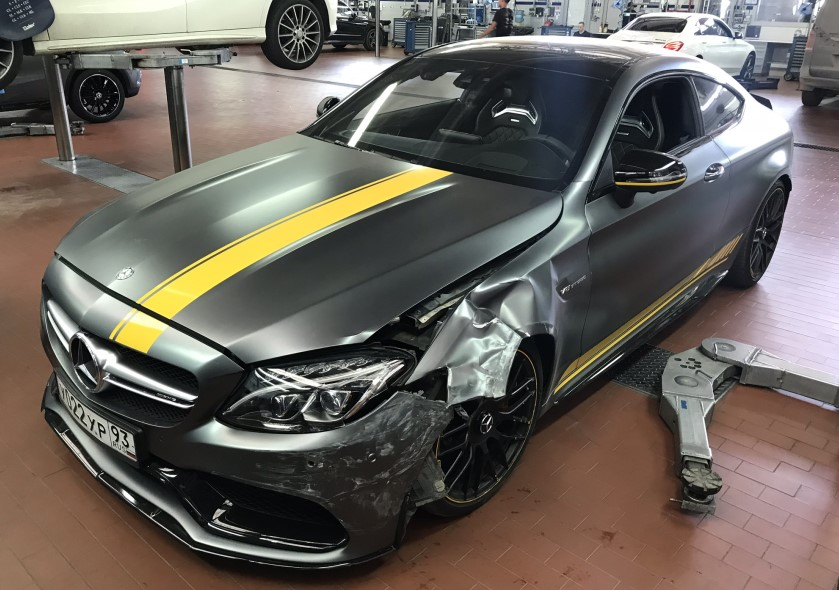
\includegraphics[width=.49\textwidth]{images/i}
		\caption{\footnotesize {Исследуемый автомобиль}}
		\label{ris:images/i}}
	\hfil \hfil%раздвигаем боксы по горизонтали 
	\parbox[t]{0.49\textwidth}
	{\centering
		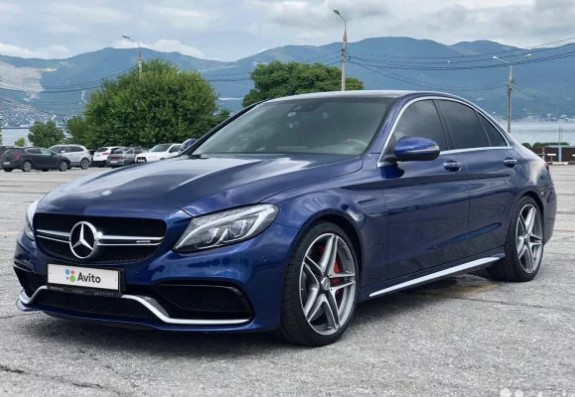
\includegraphics[width=.49\textwidth]{images/an}
		\caption{\footnotesize {Аналог 1, выбранный для оценки}}
		\label{ris:images/an}}
\end{figure}
  
  \begin{figure}[h!]\centering
  	\parbox[t]{0.49\textwidth}
  	{\centering
  		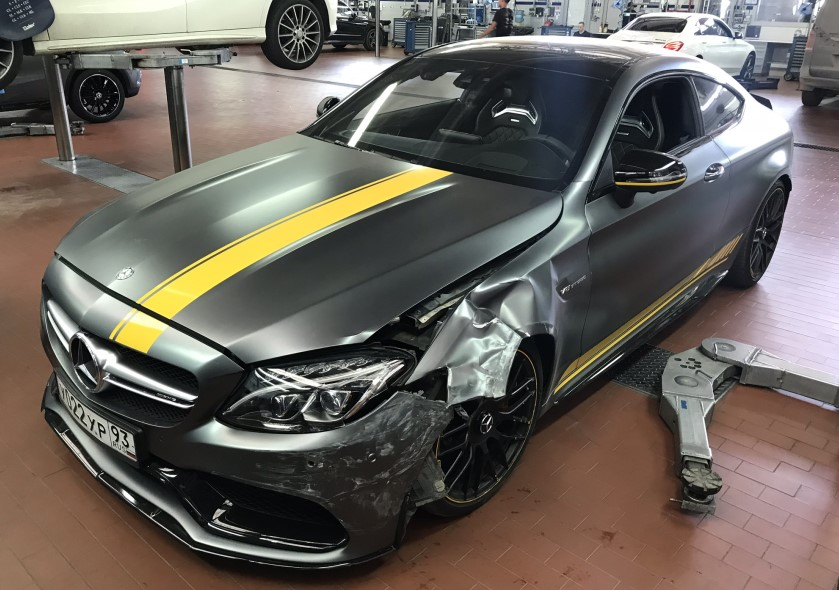
\includegraphics[width=.49\textwidth]{images/i}
  		\caption{\footnotesize {Исследуемый автомобиль}}
  		\label{}}
  	\hfil \hfil%раздвигаем боксы по горизонтали 
  	\parbox[t]{0.49\textwidth}
  	{\centering
  		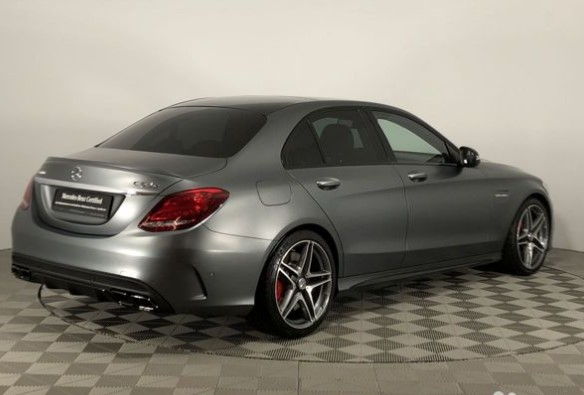
\includegraphics[width=.49\textwidth]{images/an2}
  		\caption{\footnotesize {Аналог 4, выбранный для оценки}}
  		\label{ris:images/an2}}
  \end{figure}
  
    \begin{figure}[h!]\centering
  	\parbox[t]{0.49\textwidth}
  	{\centering
  		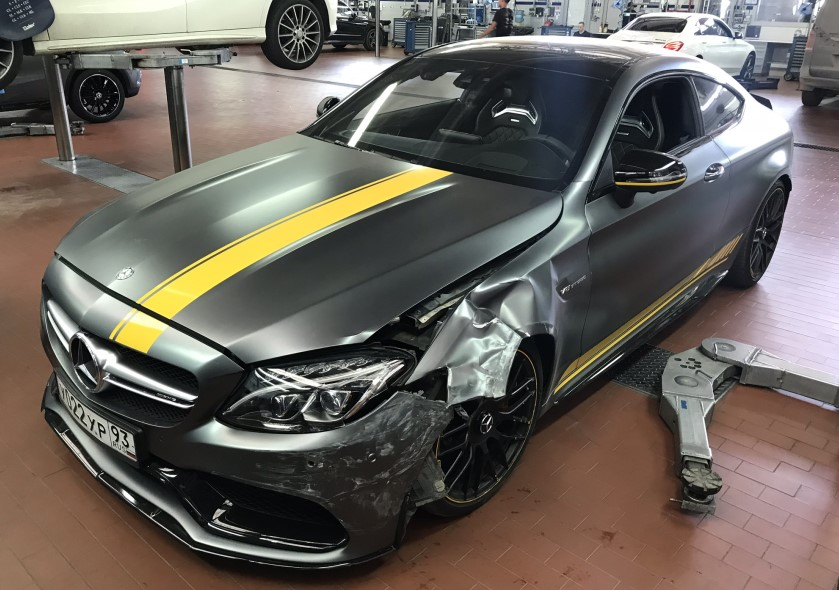
\includegraphics[width=.49\textwidth]{images/i}
  		\caption{\footnotesize {Исследуемый автомобиль}}
  		\label{}}
  	\hfil \hfil%раздвигаем боксы по горизонтали 
  	\parbox[t]{0.49\textwidth}
  	{\centering
  		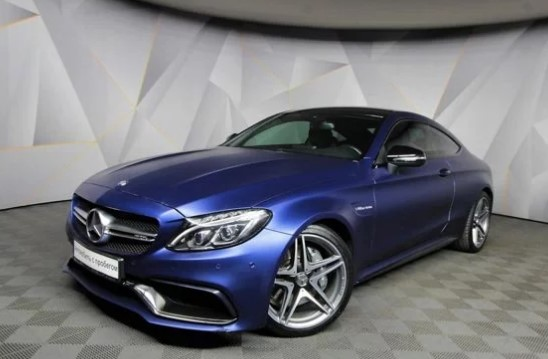
\includegraphics[width=.49\textwidth]{images/an3}
  		\caption{\footnotesize {Аналог 2, выбранный для оценки}}
  		\label{ris:images/an3}}
  \end{figure}


\par Результат выборочного анализа (3 из 5) сравнений принятых для оценки рыночной стоимости автомобилей однозначно указывает на существенное отличие выбранных аналогов от исследуемого автомобиля. Значимые различия в типе кузова, комплектации, мощности двигателя не позволяют достоверно определить рыночную стоимость исследуемого автомобиля \тс \, на основании выборки, сделанной экспертом в заключении № 00182/18.

  
  В качестве примера рецензент приводит новый, товарный, 2016 года выпуска, идентичный исследуемому автомобиль в идентичной комплектации, выставленный на продажу дилером г.  Краснодара 	«Мерседес-Бенц» Центр КЛЮЧАВТО на Красной Площади,  таблица \ref{tab:11}, по цене 8\,461\,554 (Восемь миллионов четыреста шестьдесят одна тысяча пятьсот пятьдесят четыре) рубля, \url {https://cars.mercedes-benz.ru/mobile/CarDetails/Index/443423}. Согласно расчетов эксперта \чел, уменьшение рыночной цены автомобиля \тс  более чем в два раза произошло за неполные два года эксплуатации, за безаварийный пробег менее 15000 км и находящегося на гарантийном обслуживании. Ликвидность   --50\% за два года эксплуатации вызывает сомнения в правильности расчетов. 
  
    \begin{longtable}{|p{5cm}|p{5cm}|p{5cm}|}
  	\caption[]{\footnotesize {Таблица сравнения аналогов}} \label{tab:11}\\ 
  	\hline
  	\rowcolor[HTML]{EFEFEF} 
  	Компонент сравнения & Исследуемый автомобиль& Аналог (1)  \\ \hline \endhead % повторение заголовка 
  	Объем двигателя  &4.0 & 4.0 \\ \hline
 	Модификация  &C 63 4.0 7G-Tronic (510 л.с.)  & C 63 4.0 7G-Tronic (510 л.с.)\\ \hline
  	Регион  & Краснодар  & Краснодар\\ \hline
  	Пробег, км & 12582  & 0\\ \hline
  	Год выпуска  & 2016  & 2016 \\ \hline
  	Комплектация  & Расширенный набор опций  & Расширенный набор опций \\ \hline
  	Тип кузова  & Купе  & Купе \\ \hline
  	Цена  &  -- & 8\,461\,554 \\ \hline
  	%%% ..............
  \end{longtable}
  
      \begin{figure}[h!]\centering
  	\parbox[t]{0.49\textwidth}
  	{\centering
  		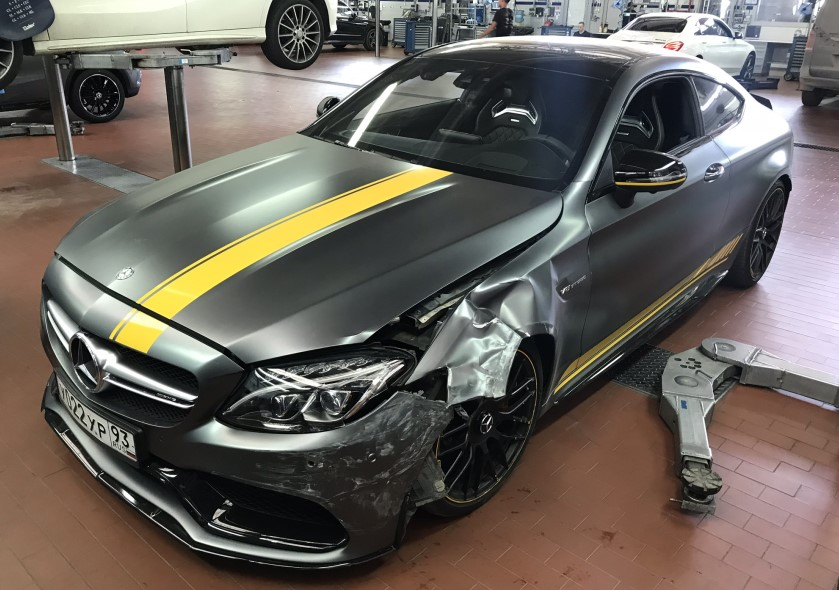
\includegraphics[width=.49\textwidth]{images/i}
  		\caption{\footnotesize {Исследуемый автомобиль}}
  		\label{}}
  	\hfil \hfil%раздвигаем боксы по горизонтали 
  	\parbox[t]{0.49\textwidth}
  	{\centering
  		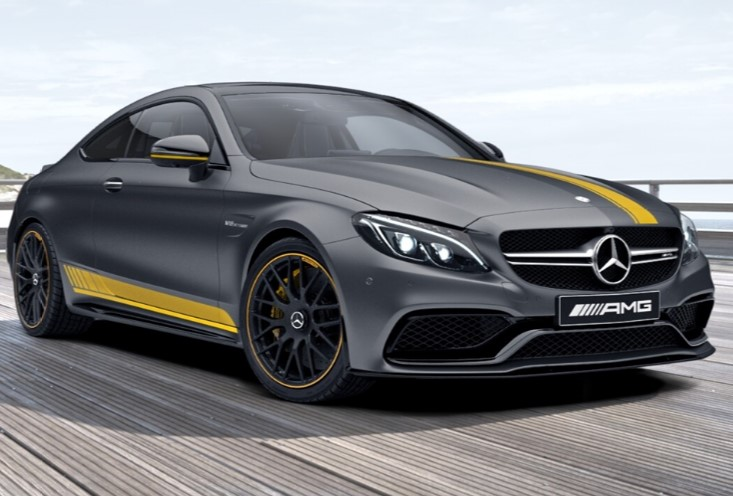
\includegraphics[width=.49\textwidth]{images/is}
  		\caption{\footnotesize {Товарный автомобиль}}
  		\label{ris:images/is}}
  \end{figure}
%  \pagebreak
  
\par Согласно заказ-наряду № ЗН19005605 от 22.06.2019 ООО "СБСВ-КЛЮЧАВТО СЕВЕР" на ремонт (дефектовка а/м после ДТП), стоимость устранения аварийных повреждений автомобиля \тс \, составляет 2\,436,843 (Два миллиона четыреста тридцать шесть тысяч восемьсот сорок три) рубля. 
\par Согласно расчетов независимой экспертизы  № 0652 от 20.06.2019 г. ООО "Фаворит", стоимость восстановительного ремонта автомобиля составляет 2\,428\,665 (Два миллиона четыреста двадцать восемь тысяч шестьсот шестьдесят пять) рублей;
\par Стоимость восстановительных расходов автомобиля, согласно рецензируемого  заключения эксперта № 00182/18  составляет 965 134 (Девятьсот шестьдесят пять тысяч сто тридцать четыре) рубля без учета износа и 857 093 (Восемьсот пятьдесят семь тысяч девяносто три) рубля с учетом износа.

Таким образом, если  разница в расчетах официального дилера изготовителя ТС и независимой экспертизой составляет менее 1\%, то разница в расчетах в сравнении с заключением эксперта составляет  более чем в 2.5 раза или 1 463 531 (Один миллион четыреста шестьдесят три тысячи пятьсот тридцать один) рубль. С целью установления причины образования столь существенной разницы, принимая во внимание вероятную разницу в стоимости детали  между розничными ценами изготовителя и указанной с справочниках РСА, рецензентом произведен сравнительный анализ повреждений автомобиля, принятых в вышеуказанных расчетах.   Результаты сравнения приведены ниже в \ref*{tab:sravnenie}.


{\footnotesize \
\begin{longtable}{|p{1.5in}|p{1.5in}|c|c|p{1.5in}|c|c|p{1.5in}|c|}
\caption{\footnotesize {Сводная сравнительная таблица поврежденных деталей}}
\label{tab:sravnenie}\\ \hline
\textbf{Наименование детали} & \textbf{Заключение эксперта} & \textbf{Акт осмотра ООО "Фаворит"} & \textbf{Дилер Мерседес} \\ \hline \endhead
Крыло переднее левое & \bullet & \bullet&\bullet \\ \hline 
Облицовка бампера переднего & \bullet& \bullet&\bullet \\ \hline 
Дверь левая & \bullet& \bullet& \bullet\\ \hline 
Шумоизоляция двери & \bullet &   &\bullet \\ \hline 
Фара левая & \bullet& \bullet&\bullet \\ \hline 
Капот & \bullet& \bullet& \bullet\\ \hline 
Диск переднего левого колеса & \bullet & \bullet&\bullet \\ \hline 
Шина переднего левого колеса & \bullet& \bullet&\bullet \\ \hline 
Облицовка арки переднего левого колеса & \bullet& \bullet& \bullet\\ \hline 
Облицовка переднего бампера левая & \bullet & \bullet&\bullet \\ \hline 
Накладка защитная переднего бампера левая& \bullet& \bullet&\bullet \\ \hline 
Усилитель передний & \bullet& \bullet& \bullet\\ \hline 
Балка переднего моста & \bullet & \bullet&\bullet \\ \hline 
Управление рулевое & \bullet& \bullet&\bullet \\ \hline 
Амортизатор передний левый & \bullet& \bullet& \bullet\\ \hline 
Стабилизатор передний & \bullet & \bullet&\bullet \\ \hline 
Насос омывателя & \bullet& \bullet&\bullet \\ \hline 
Шланг омывателя & \bullet& \bullet& \bullet\\ \hline 
Усилитель переднего бампера & \bullet & \bullet&\bullet \\ \hline 
Буфер передний левый & \bullet& \bullet&\bullet \\ \hline 
Радиатор левый & \bullet& \bullet& \bullet\\ \hline 
Желоб передний левый & \bullet & \bullet&\bullet \\ \hline 
Датчик ускорения передний левый & \bullet& \bullet&\bullet \\  \hline 
Датчик парковки передн. нар. лев. & \bullet & \bullet&\bullet \\ \hline 
Датчик парковки передн. вн. лев. & \bullet& \bullet&\bullet \\  \hline 
 Поперечная тяга левая &  --- & \bullet& \bullet\\ \hline 
 Панель передка  & --- & \bullet&\bullet \\ \hline 
 Шина передняя левая & ---& \bullet&\bullet \\ \hline 
 Лонжерон передний левый &--- & \bullet& ---\\ \hline 
 Тормозной диск передний левый& --- & \bullet&\bullet \\ \hline
 Тормозной диск передний правый&  ---& \bullet&\bullet \\ \hline  
 Стабилизатор  & --- & \bullet&\bullet \\ \hline 
Порог внутренний левый  & --- & \bullet& \bullet\\ \hline 
Уплотнитель передней левой двери  & --- & ---&\bullet \\ \hline 
 Молдинг крыши слева &---& ---&\bullet \\ \hline 
 Шильдик V8 Biturbo слева &---  & --- &\bullet \\ \hline 
 Стойка переднего стабилизатора слева&---  & --- &\bullet \\ \hline
 Уплотнитель между крылом и дверью слева&---  & --- &\bullet \\ \hline
Кронштейн переднего бампера левый &---  &--- &\bullet \\ \hline
Электропроводка бампера & --- & \bullet&\bullet \\ \hline

\end{longtable}}
\noindent \bullet -- деталь присутствует в перечне повреждений \\
--- деталь отсутствует в перечне повреждений.

Приведенная таблица \ref*{tab:sravnenie}  наглядно иллюстрирует то, что в заключении эксперта № 00182/18 отсутствует часть деталей, присутствующая в акте осмотра  автомобиля \тс \, № 0652 от 20.06.2019 г. ООО "Фаворит" и в заказ-наряде № ЗН19005605 от 22.06.2019 ООО "СБСВ-КЛЮЧАВТО СЕВЕР" на ремонт (дефектовка а/м после ДТП). При этом, эксперт \чел в своем заключении не представил обоснования исключения деталей из расчета.
\par С целью определения степени влияния на итоговые результаты исследования,  рецензентом был выполнен расчет стоимости замены некоторых  исключенных позиций: жгута бампера, надписи крыла переднего левого, уплотнителя двери, тяги рычага левого, шины передней левой, тормозного диска. Расчет производился   в специализированном программном продукте, содержащем нормативы трудоёмкости работ, регламентируемые изготовителями транспортного средства     AudaPadWeb, лицензионное соглашение № AS/\- APW-658  RU-P-409-409435. \\[3mm]
%
% Идентификационный код автомобиля (VIN)  \vin \, содержит следующую информацию о транспортном средстве, имеющую значение для 	дачи заключения:
% 
\begin{figure}[H]
	\centering
	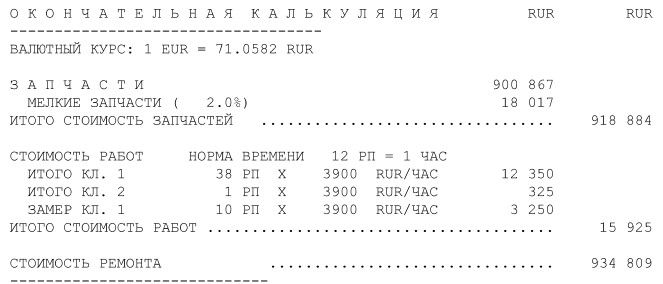
\includegraphics[width=0.8\linewidth]{images/itog}
	\caption[]{Итоговый расчет 934 809 руб.}
	\label{fig:itog}
\end{figure}

\noindent Калькуляция выполнена при следующих допущениях:\\
-- возникшие правовые отношения  регулируются Гражданским кодексом РФ;\\
-- стоимость коммерческого нормо-часа работ применена  с учетом условий регионального рынка услуг и сложившихся средних расценок по видам работ, типу ТС, а также по маркам и моделям ТС  и   составляет 3900 р/ч для данного транспортного средства. Трудоёмкость работ по разборке/сборке/замене  соответствует трудоемкости работ, рекомендованной заводом изготовителем ТС. Расчет стоимости ремонта, согласно положениям Методики [2] производится с учетом  применения оригинальных запасных частей, которые поставляются изготовителем КТС авторизованным ремонтным организациям. Техническое состояние запасных частей учитывается коэффициентом износа \footnote{Согласно п. 7.8.\, Методики [2]  для случаев, не регулируемых законодательством об ОСАГО, для составных частей КТС значение износа принимается равным нулю если  срок эксплуатации КТС не превышает пяти лет, иные повреждения и следы ремонта отсутствуют, признаки интенсивной эксплуатации отсутствуют }, что в совокупности с установкой оригинальных запасных частей в максимальной степени отвечает понятию «восстановительный ремонт», то есть восстановления состояния КТС, при котором используются установленные изготовителем составные части, но с использованным частично ресурсом.\\
В результате произведенного расчета получено значение  стоимости ремонта исключенных экспертом деталей автомобиля \тс,\, составляющее  934 809 рублей и превышающее стоимость восстановительного ремонта с учетом износа (857 093 рубля) согласно заключению эксперта № 00182/18.\\
\indent Таким образом,  исключенные экспертом детали оказывают существенное влияния на итоговые результаты исследования. Добавление жгута бампера, надписи крыла переднего левого, уплотнителя двери, тяги рычага левого, шины передней левой, тормозного диска в совокупности с учетом требований изготовителя по замене парных деталей приводят к увеличению стоимости ремонта вдвое.


\section{ Анализ представленных экспертом выводов}

Вывод эксперта о стоимости восстановительного ремонта автомобиля \тс \, основывается на перечне поврежденных деталей, из которого экспертом \чел не\-обосновано  исключены поврежденные дорогостоящие детали, является неполным и недостоверным.

Вывод эксперта о рыночной стоимости транспортного средства   на момент ДТП в исправном техническом состоянии основывается на не полных аналогах, имеющих существенные отличия от исследуемого автомобиля \тс. \, Следовательно, определенная экспертом \чел величина рыночной  стоимости является недостоверной и ведет к ошибкам в определении зависимым от нее величинам. 

Вывод эксперта о величине утраты товарной стоимости автомобиля \тс \, сделан экспертом на основании произведенных расчетов, основанных на сведениях о виде, характере и объеме повреждений и ремонтных воздействий, а так же на значении рыночной стоимости автомобиля.   
\par Величина УТС ( $ C_\text{YTC} $)  определяется на дату оценки (исследования) по формуле: 

\begin{equation}\label{uts}
C_{YTC} = C_{KTC} \cdot \dfrac{\sum К_{УТСi}}{100\%}, \text{руб.},
\end{equation}

\noindent $ C_{KTC} $ -- стоимость КТС на дату оценки (исследования), руб;\\
$ K_{YTCi} $ -- коэффициент УТС по i-му элементу КТС, ремонтному воздействию, \%. 
\par Значения коэффициентов УТС ($ C_{KTC} $) определены по результатам экспертой практики и приведены в приложении [2,Приложение 2.9].

\par Так как величина утраты товарной стоимости прямо пропорциональна рыночной стоимости  автомобиля, количеству и степени повреждений автомобиля, то в случае неверного, ошибочного определения рыночной стоимости  транспортного средства расчитанная величина  УТС  так же  является недостоверной.
 


\subsection{ ОЦЕНКА ЗАКЛЮЧЕНИЯ}


Заключение эксперта должно основываться на положениях, дающих возможность проверить обоснованность и достоверность сделанных выводов на базе общепринятых научных и практических данных. Исследование, результаты которого изложены в представленном заключении, не является полным, всесторонним и объективным, что противоречит действующим требованиям о том, что заключение должно быть объективным, обоснованным и полным (то есть, содержать исчерпывающие ответы на поставленные вопросы), всесторонним, тщательным, проводиться в пределах специальности эксперта, на строго научной и практической основе с использованием современных достижений науки и техники. Ответы на поставленные вопросы не являются исчерпывающими, выводы эксперта не обоснованы и вызывают сомнение в правильности.


\subsection{ ВЫВОД}

Заключение эксперта № 00182/18 по гражданскому делу № 2-802/19 по иску Хачатряна Андраника Гайковича к Мокину Игорю Витальевичу о возмещении материального ущерба, причиненного дорожно-транспортным происшествием произведено с нарушениями действующего законодательства, методических рекомендаций проведения данного вида исследований и вызывают сомнения в компетентности эксперта,  что является основанием для назначения повторной судебной автотехнической экспертизы.\textbf{}
\vspace{7mm}
\relax
Приложение:\\
\vspace{3mm}
\textit{\small 
\noindent	Приложение № 1. Расшифровка модельных опций ТС \тс \\
%	Приложение № 1. Акт осмотра ТС \тс\\
%	Приложение № 2. Фототаблица повреждений ТС \тс\\
	Приложение № 3. Калькуляция стоимости восстановительного ремонта ТС \тс\\
%	Приложение № 4. Цифровые копии регистрационных документов ТС\\
%	Приложение № 5. Цифровая копия постановления по делу об административном правонарушении дорожно-транспортном происшествии\\
	Приложение № 6. Правоустанавливающие документы\\}


\vspace{15mm}


\noindent Рецензент \hfill  \underbar{ }Мраморнов А.В.

\vspace{20mm}

\input bibliography

%\includepdf[pages=-]{foto.pdf}
\includepdf[pages=-]{myfile.pdf}
%\includepdf[pages=-]{calc.pdf}
